\documentclass{article}
\usepackage{times}
\usepackage{graphicx}

\newcounter{lastnumber} %For continuation of enumerated lists

\begin{document}

\noindent {\Huge \bf A Proposed Hazard Modelling Project within
the Risk Research Group}

\medskip
\textit{Draft dated 28/7/2003 11:00am}


\section{Background}

This proposal describes the development of a \textit{generic rapid
onset hazard model} which will form the basis for a collection of
software aimed at specific hazard models. Lacking a better name, we
will refer to this framework as GROHM in the following.

The GROHM is based on the theory of fluid mechanics and is aimed at 2D
processes that can be described in terms of conservation laws. The
GROHM will be capable of simulating a range of physical processes on
realistic complex topologies and will be suitable for the detailed
modelling of natural hazards such as tsunamis, landslides, estuarine
environmental modelling, riverine processes
such as sediment transport and flooding, avalanches, explosions, and 
storm surges which are wind driven events leading to flooding of
coastal regions. The storm surge model will form a prototype for
developing other hazard models using the GROHM framework.


The GROHM software can be used in-house in a risk modelling context but can
also be made available to consultants/councils who may not
have the expertise or funds to develop their own models.

Main participants in this project are 
Chris Zoppou, Duncan Gray, Miriam Middelman, Ole Nielsen, Stephen Roberts.

\section{Relevance to a larger risk modelling framework}


Generally, a risk assessment consists of
\begin{itemize}
  \item A physical model for the hazard in question.
  The GROHM framework applies to this item.
  \item The degree of exposure of people and infrastructure
  \item The vulnerabilities (social, economical and environmental)
  of the exposed entities.
\end{itemize}

The GROHM model will initially be focused on storm surge hazard
modelling with a view to incorporating the model into the broader
risk modelling framework.

\section{Reasons for developing the GROHM model.}

Most hazard modelling approaches have so far generally been based on ad-hoc
methodologies. For example, deficiencies in current storm surge hazard
modelling approaches include
\begin{itemize}
  \item Inability to include wetting and drying processes of shorelines
  \item Reliance on of the Holland model for cyclone wind fields.
  The Holland model is very crude and more sophisticated approaches exist.
  %FIXME: Is it inadequate??
  \item Modelling topologies on Cartesian grids which do not capture
  realistic complex topographies and bathymetries.
\end{itemize}
A storm surge model based on GROHM will overcome these deficiencies.

Moreover, some hazards for which no model exists at present 
(e.g.\ simulation of landslides or flash flooding) 
can be modelled using GROHM. In addition, GROHM will be
applicable to other hazards such as tsunamis, estuarine
environmental modelling, avalanches, explosions, riverine
processes such as sediment transport and flooding.

However, the GROHM, being a 2D model, will not be suitable for the
modelling of geophysical hazards such as earthquakes and
volcanoes, or atmospheric hazards such as synoptic storm fronts or
hail. Nor will it be able by itself to model the exposures,
vulnerabilities or economics needed in the broader risk modelling
process. It will however, be an integral component in such a risk
modelling framework.


\section{Model development options}
Broadly, there are two options for the model development; it can
be done in-house or by consultants.  Having the consultants
develop the model will be costly.  Furthermore, the research
needed to develop GROHM is outside the expertise of most software
consultants.  Although there are engineering consultants that may
have the expertise to develop models for specific hazards, they
may not have the expertise in developing a single modelling
framework for multiple hazards and integrating the framework into
a risk modelling framework.

If it is developed in-house we will have more control and
understanding on the model development and implementation.
Additionally, in-house development will increase our experience in
the cost of model development and will also provides the RRG the
opportunity to cement RRG as a leader in hazard scenario
prediction as well as risk assessment.

Developing a single model capable of simulating several hazard types means that the RRG only need to understand the idiosyncrasies of one single tool
instead of several which would be the case for commercially developed model
that address one single hazard.
This also has implications in setting down data standards.
This task will be easier if the RRG has the control of both data and tools.


\section{Essential components}

We have identified a number of separate but interdependent components which, 
together, will constitute GROHM.

\begin{enumerate}
\item Finite Volume code.  Solves conservation laws such as water,
  avalanche, landslide and tsunami evolution on arbitrary domains. A
  prototype is available in Matlab for the shallow water wave
  equations and algorithms are currently being further developed for
  generic conservation laws that describe a broader class of hazards.
  \label{item:FV}
\item Triangulation (mesh generation) e.g. bathymetry, topography as
  well as buildings. This work is in progress.
  \label{item:TIN}
\item Random field generator - e.g. to capture uncertainties in
  spatial parameters values. An example is the \textit{Mannings
  roughness coefficient} $n$.  A random field generator can generate a
  distribution of parameters for use with Monte Carlo simulations.
  \label{item:RAND}
\item Visualisations, e.g.\ Computational fluid dynamics animations or
  maps with inundations of buildings and infrastructure displayed.
  \label{item:VIZ}

\setcounter{lastnumber}{\theenumi}
\end{enumerate}

These components are essential for the hazard impact prediction
component of GROHM.
Other components required will depend on the
specific hazard being considered. Two examples are provided
below.

\section{Risk assessment modelling framework}

The two remaining components required by the GROHM framework to
undertake risk assessment is the need for a:
\begin{enumerate} 
 \setcounter{enumi}{\thelastnumber}
\item building vulnerability model, and
  \label{item:VULN}
\item economic loss model.
  \label{item:ECO}
\setcounter{lastnumber}{\theenumi}  
\end{enumerate} 

\section{GROHM components needed for the storm surge model}

For a full storm surge model, the following GROHM components will
also be needed.

\begin{enumerate}
 \setcounter{enumi}{\thelastnumber}
\item Mapping: Georeferencing (Northings and eastings or latitudes and
  longitudes) to a triangular mesh (e.g. to describe movement of cyclone).
  \label{item:MAP}
  Codes from a GPS application are available and will serve as a
  starting point.
\item Tidal model to provide a boundary condition.
  Hopefully, this can be provided by the Bureau of Meteorology.
  \label{item:TIDAL}
\item A computationally efficient cyclone model to provide forcing function (generates winds).
  A number of alternatives are
  \begin{itemize}
    \item The Holland model (most basic, available)
    \item Keppert model (more sophisticated, available)
    \item Warburton model (most sophisticated, being developed)
  \end{itemize}
  \label{item:CYCLONE}
\setcounter{lastnumber}{\theenumi}
\end{enumerate}


Figure \ref{fig:flowchart} illustrates the interplay among the
components described above.
\begin{figure}
  \begin{center}
    %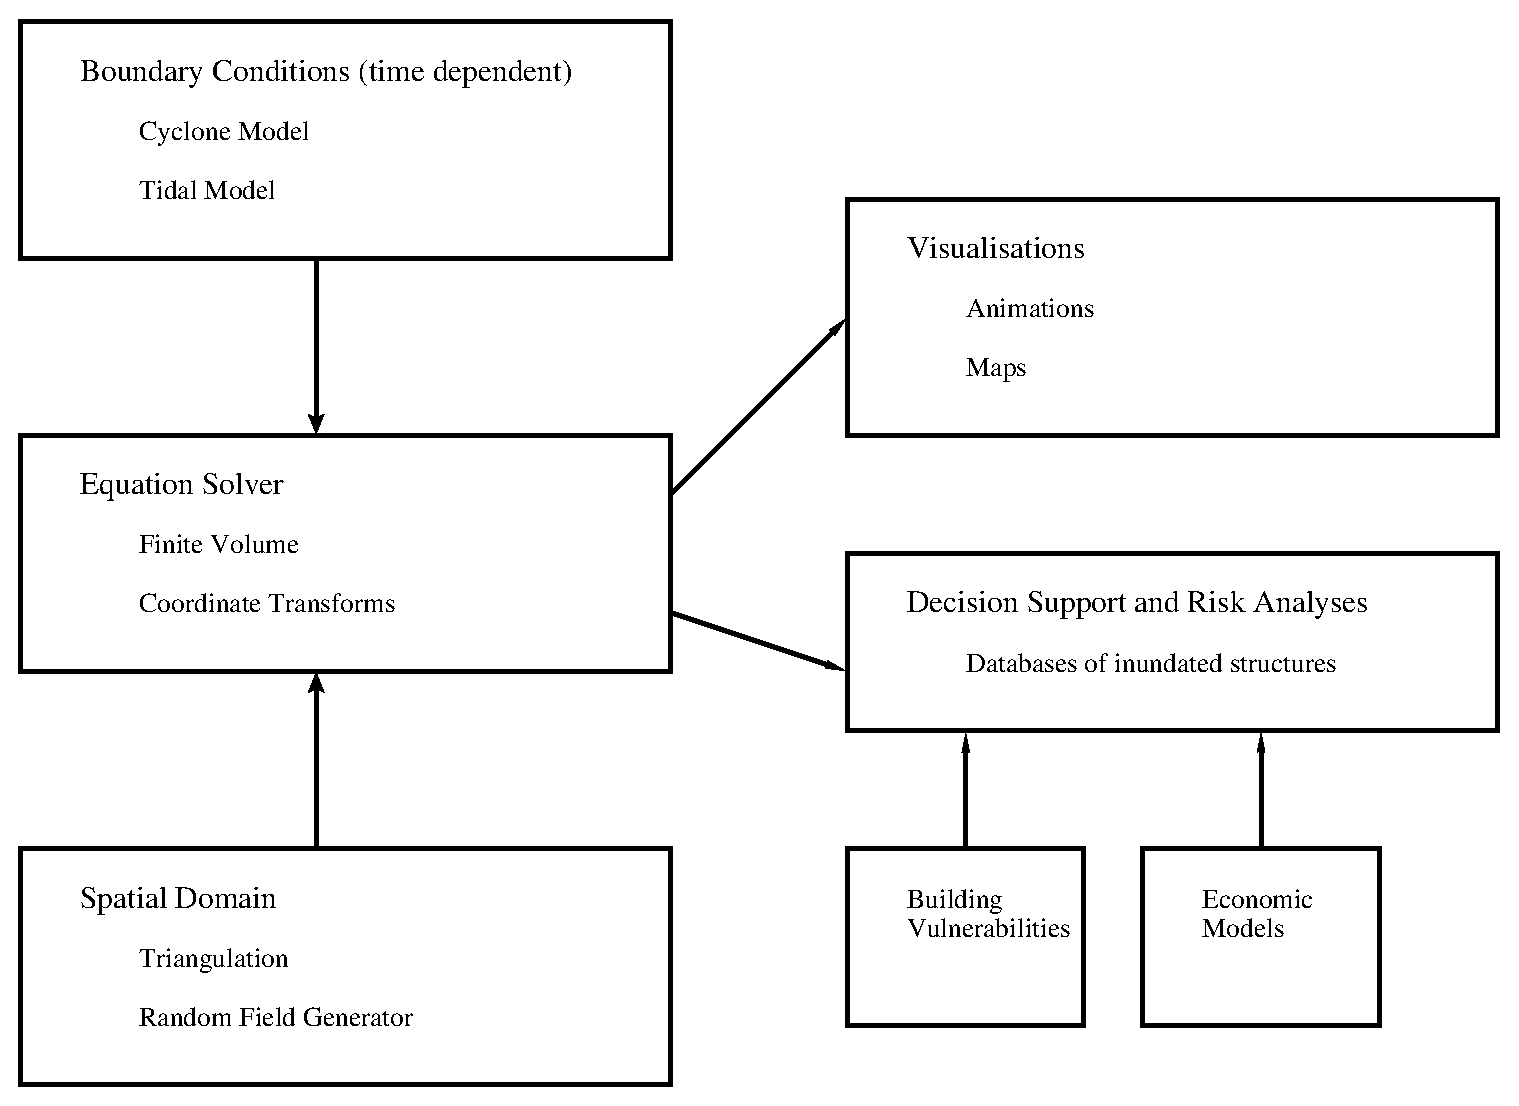
\includegraphics[width = 0.9\textwidth]{hazard_modelling_flowchart}
    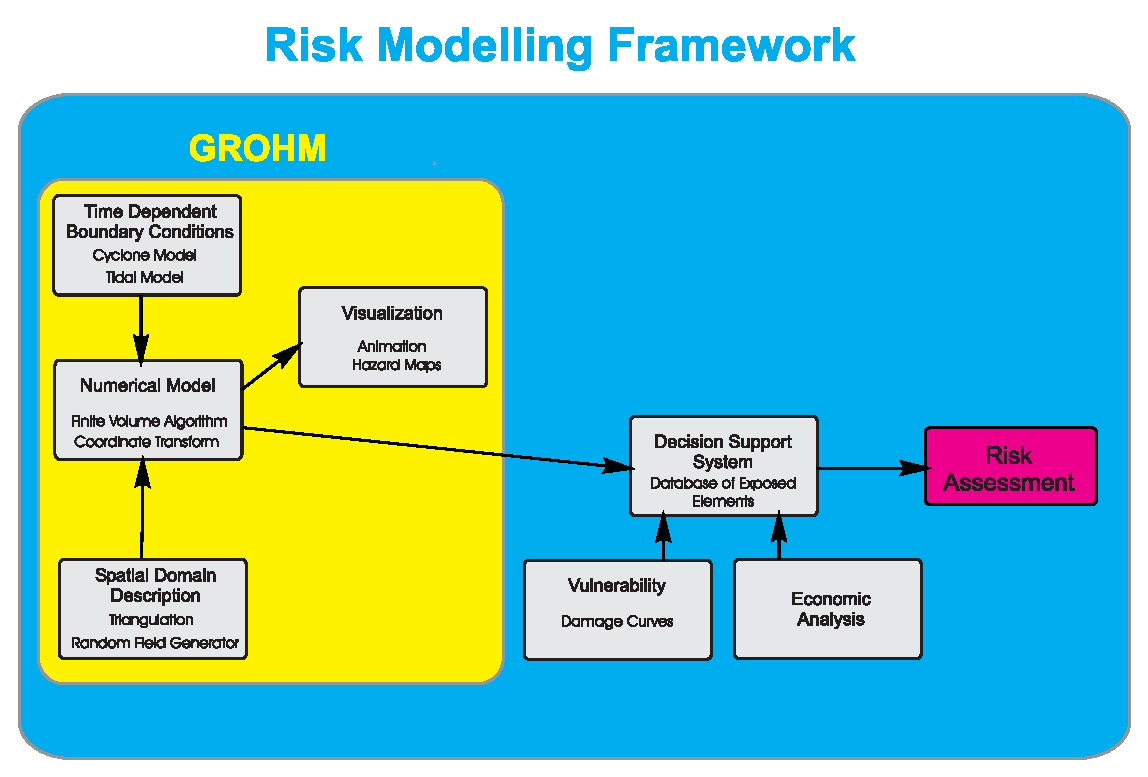
\includegraphics[width = 0.99\textwidth]{GROHM}    
  \end{center}

  \caption{GROHM components for risk analysis of storm surges.}
  \label{fig:flowchart}
\end{figure}

\section{GROHM components needed for riverine flooding risk assessment}

Several components of the storm surge model are also relevant to
the riverine model. These include;

\begin{itemize} 
   \item Tidal model (\ref{item:TIDAL}) 
   \item Random field model (\ref{item:RAND}) 
   \item Visualisation (\ref{item:VIZ})   
   \item Building vulnerability, which includes the duration, velocity and depth of inundation (\ref{item:VULN})  
   \item Economic loss (\ref{item:ECO})   
\end{itemize} 

With the addition of the hazard model, in this case an unsteady
flow model, then the required components for risk assessment of
riverine flooding will be available.


\pagebreak
\section{Tasks and responsibilities}
\noindent\textbf{Deliverables by 30 June 2004 and Specific Activities}:

%
% Names have been commented out until we decide who'd doing what
%
\begin{itemize}
\item Graphical triangulation software (\ref{item:TIN}) for describing
the two dimensional topography/bathymetry by a triangular mesh.  
%DG \& CZ

  \begin{itemize}
      \item engine for generating high quality meshes.
      \item user interface to the triangulation program for
      importing external point data files, editing, inserting points,
      refining the triangular grid, zooming and executing the
      triangulation package.
      \item graphical boundary condition interface for the storm surge model.
      \item export facility for including the mesh and associated data in
      the required formats for the finite volume code and reports.
      \item demonstration of the versatility of the mesh generator for tropical
      cyclone Vance data and its complex geometry.
      \item Open source distribution of the developed module.
  \end{itemize} 

  \item Finite Volume code (\ref{item:FV}) This is the core of the GROHM
  framework.  This component will solve the underlying equations using
  a finite-volume scheme and output values of the target variable for
  each point in the mesh.
  \begin{itemize}
      \item alternative to the existing Riemann solver for
      inclusion in the finite volume code that is capable of handling
      any system of conservation laws.
      \item solver for discontinuous terrain.
      \item solver for stiff source terms.      
      \item Investigation of how higher order terms (Boussinesq terms) can be
      incorporated into the shallow water wave equations (1-D problem)
      \item investigation of the conservation of energy and momentum problem.
  \end{itemize}
  %Applicable for storm surge, estuarine flooding,
  %flash flooding, avalanches, landslides and explosives.
  %Concentrate on first two initially.

  %CZ, SR \& ON
  \item Boundary conditions
    ( \ref{item:MAP}, \ref{item:TIDAL} \& \ref{item:CYCLONE})
  \begin{itemize}
    \item general and modular methodology for applying boundary conditions
    to the solver
    \item program to convert Latitudes and Longitudes into model
    co-ordinates
  \end{itemize}
  \item General models that represent forcing functions for the the solver
  %CZ, NM, MM
  \begin{itemize}
  \item cyclone wind field model
  \item wind shear model
  \item tidal cycle model 
  \end{itemize}
\item
  Visualisation (\ref{item:VIZ})
  \begin{itemize}
    \item Assessment of visualisation needs with a view to presenting
      hazards and risks both spatially and temporally.
    \item integration of GIS into the GROHM framework
    \item ability to animate results produced from the
      finite volume model    
    \item other visualisation components as appropriate
  \end{itemize}

  %DG \& ON
  %\item A storm surge model based on the GROHM components.
\end{itemize}

\noindent\textbf{Beyond 1 July 2004}:
\begin{itemize}
  \item Model validation
  \item Application of storm surge model to real scenarios
  \item Decision support system (based on ideas from
    Andre Zerger) incorporating the other elements of risk analysis
    namely exposure, vulnerability and economics.
  \item Random field generator (\ref{item:RAND})
  \item Computation and visualisations of detailed structure response to
  water waves (\ref{item:VIZ}).
\end{itemize}


\section{Summary}

It is the intention of the RRG to develop a prototype GROHM framework
which will integrate a single hazard modelling methodology that
will be capable of predicting the impact from a number of hazards
within a risk modelling framework. The proposal also links the
development of advanced rapid onset hazard models with decision
support systems. Storm surge modelling has been selected as the
prototype hazard.

\end{document}
